\chapter{Introduction}
\label{ch:intro}

\begin{figure}[H]%
\begin{center}
%
  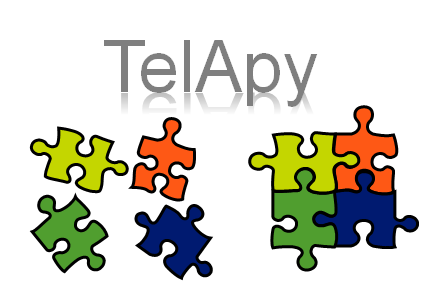
\includegraphics[width=0.8\textwidth]{./Figures/TelApy.png}
%
\end{center}
\label{fig:telApy}
\end{figure}

This guide aims to explain the use of the \TelApy{} module
of the \telemacsystem. This module aims to provide python control of \tel{} API
(Application Program Interface).

The API’s main goal is to have control on a simulation while running a case.
For example, it must allow the user to stop the simulation at any time step,
retrieve some variable values and change them. In order to make this possible,
a \fortran{} structure called instance is used in the API\@. It contains a
list of variables declared as pointers that are pointing to variables.
This gives direct access to the physical memory of variables, and allows
therefore to retrieve their values, and modify them. Furthermore, based on modifications
in \tel{} main subroutines, it is possible to run hydraulic case time step by time step.

Thus, the APIs development allows the interoperability of the \telemacsystem{}
modules. Interoperability is the ability of a computer system to operate with
other existing or future informatic products without restricting access or
implementation.
It, then, becomes natural to drive these APIs using Python programming
language. In fact, Python is a portable, dynamic, extensible, free language,
which allows (without imposing) a modular approach and object oriented
programming. Python has been developed since 1989 by Guido van Rossum and many
volunteer contributors. In addition of the benefits of this programming
language, Python offers a large amounts of interoperable libraries. The link
between various interoperable libraries with \telemacsystem{} APIs allows the
creation of an ever more efficient computing chain able to more finely respond
to various complex problems.

Consequently, the TelApy module has the ambition to facilitate the usage of
\telemacsystem{} for optimization, coupling, uncertainty quantification\ldots
applications.
